%!TEX root=../document.tex

\section{Einführung}
\label{sec:intro}

Das folgende Dokument befasst sich mit Datamining (auch als knowledge discovery from data oder KDD bekannt).  Im heutigen Zeitalter sind wir mit enormen Mengen an Informationen anhand von Daten umgeben. Der Markt produziert weltweit eine gigantische Anzahl an Information bezüglich Finanzgeschichte, Produktbeschreibungen, Performance Logs, Kundenfeedback und vielem mehr. 

Eine Suchmaschine (z.B. Google) erhält hunderte von Anfragen jeden Tag. Jede einzelne dieser Anfragen kann als Transaktion gesehen werden. Bei dieser Transaktion beschreibt der Verwender, welche Information er erhalten will. Bei Datamining geht es unter anderem auch darum Informationen aus Daten zu erhalten die nicht offensichtlich sind und bei welchen Algorithmen mehr rausholen können. So könnten Algorithmen mit den Anfragen an Google den Wohnort, Beziehungsstatus, Alter und vieles mehr.

In Abbildung \ref{fig:dbevolution} kann gesehen werden wie Datamining klassifiziert ist und in welcher Beziehung es zu anderen Konzepten des Datenmanagement steht.

\begin{figure}[!h]\centering
	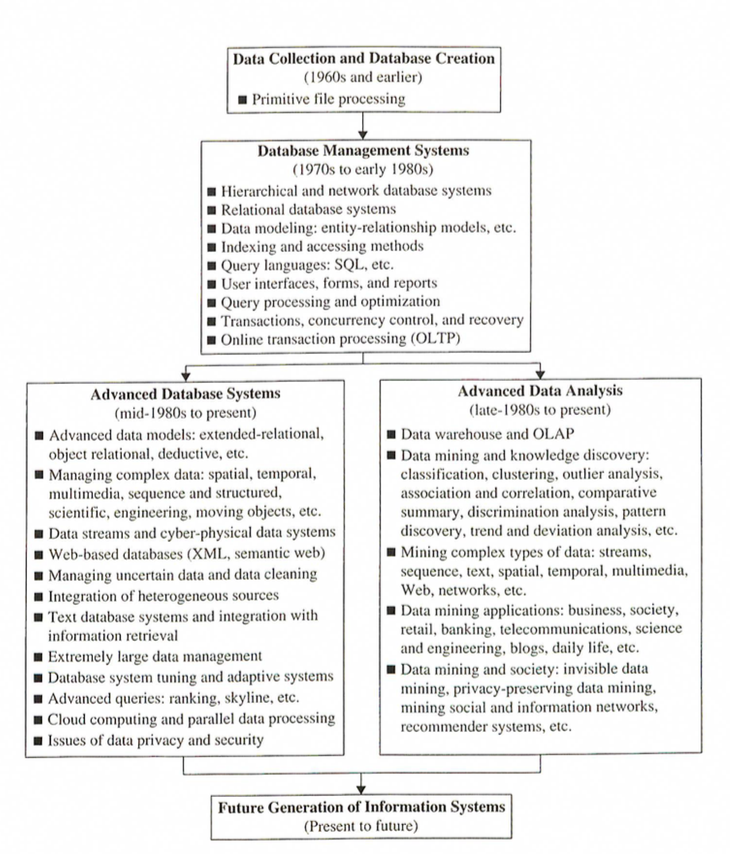
\includegraphics[width=0.6\textwidth]{images/dbevolution}
	\caption{Entwicklung von Datenbank Technologien \cite{DataMiningConceptsAndTechniques}}
	\label{fig:dbevolution}
\end{figure}